%% ============================================================================
%% Paper 2: Estimand Divergence: Static Docking Versus Dynamics for Antimalarial Triage
%% ChemRxiv Preprint Version (converted from JCIM achemso format)
%% Article source — September 2026 (V2609C: literature-integrated reframing)
%% ============================================================================

\documentclass[11pt,a4paper]{article}

\usepackage[margin=1in]{geometry}

% Fonts and encoding
\usepackage[T1]{fontenc}
\usepackage[utf8]{inputenc}
\usepackage{lmodern}

% Mathematics
\usepackage{amsmath, amsfonts, amssymb, mathtools}

% Figures and tables
\usepackage{graphicx}
\usepackage{booktabs, tabularx, array, multirow, longtable}
\usepackage{tikz}

% ORCID icon defined locally for the article class
\providecommand{\textorcid}{%
	\begin{tikzpicture}[baseline=0.0ex,line width=0.6,scale=0.65]
		\fill[rounded corners=0.5,fill=green!60!black,draw=green!50!black] (0,0) circle (0.65ex);
		\node[white,font=\bfseries\sffamily\tiny] at (0,0) {iD};
	\end{tikzpicture}%
}

\usepackage{rotating}
\usepackage[table]{xcolor}
\usepackage[labelfont=bf,textfont={footnotesize,it}]{caption}
\usepackage[colorlinks=true,linkcolor=blue,citecolor=blue,urlcolor=blue]{hyperref}
\usepackage{microtype}
\usepackage[numbers,sort&compress]{natbib}

% Units and SI
\usepackage[
  group-minimum-digits = 5,
  per-mode             = symbol,
  range-phrase         = {--},
  range-units          = single,
  separate-uncertainty = true,
  retain-explicit-plus = true,
]{siunitx}
\DeclareSIUnit\molar{M}
\DeclareSIUnit\angstrom{\text{\AA}}
\DeclareSIUnit\kcalmol{kcal\,mol^{-1}}
\DeclareSIUnit\barpressure{\mathrm{bar}}

% Cross-referencing
\usepackage[nameinlink,noabbrev]{cleveref}
% SM cross-refs (labels SM-* live in the supplementary document)
\usepackage{xr}
\externaldocument[SM-]{P2_MD_Validation_ChemRxiv_SM}

% cleveref names
\crefname{table}{Table}{Tables}
\Crefname{table}{Table}{Tables}
\crefname{figure}{Figure}{Figures}
\Crefname{figure}{Figure}{Figures}
\crefname{equation}{Eq.}{Eqs.}
\crefname{section}{Section}{Sections}
\crefname{subsection}{Section}{Sections}

% Path configuration
\graphicspath{{Graphics/}}

% ============================================================================
% TITLE AND AUTHOR INFORMATION
% ============================================================================

\title{Estimand Divergence: Static Docking Versus Dynamics for Antimalarial Triage}

\date{}

% ============================================================================
% BEGIN DOCUMENT
% ============================================================================

\begin{document}

{\centering\Large\bfseries Estimand Divergence: Static Docking Versus Dynamics for Antimalarial Triage\par}
\vspace{1em}
{\centering
	Myke Vital Sao Temgoua\href{https://orcid.org/0009-0004-5170-2309}{\textsuperscript{\textorcid}}\footnotemark[1]$^{1}$,
	Jean-Pierre Tchapet Njafa\href{https://orcid.org/0000-0002-1936-8353}{\textsuperscript{\textorcid}}$^{1}$,
	Penabei Samafou\href{https://orcid.org/0000-0002-9683-7678}{\textsuperscript{\textorcid}}$^{2}$,
	Wilfred Fon Mbacham\href{https://orcid.org/0000-0002-3934-3233}{\textsuperscript{\textorcid}}$^{3}$,
	Serge Guy Nana Engo\href{https://orcid.org/0000-0002-7484-3508}{\textsuperscript{\textorcid}}$^{1}$\\[0.5em]
	{\small $^{1}$Department of Physics, Faculty of Science, University of Yaound\'e I, P.O. Box 812, Yaound\'e, Cameroon}\\
	{\small $^{2}$Department of Medical Imaging and Radiation Sciences, Universit\'e de Sherbrooke, Sherbrooke, QC, Canada}\\
	{\small $^{3}$Department of Biochemistry, Faculty of Science, University of Yaound\'e I, P.O. Box 812, Yaound\'e, Cameroon}\par}

\footnotetext[1]{Corresponding author: \texttt{myke-vital.sao@facsciences-uy1.cm}}

% ============================================================================
% GRAPHICAL TABLE OF CONTENTS (mandatory for ACS/JCIM submission)
% ============================================================================


% ============================================================================
% ABSTRACT


% ============================================================================

% ============================================================================
% ABSTRACT
% ============================================================================

\begin{abstract}
We evaluated a multi-target docking framework in \num{136} docking systems spanning wild-type and mutant PfDHFR/PfCRT states, built from 396 African natural products and 454 synthetic antimalarials. A Resistance-Resilience Score stratified the primary cohort ($n=\num{12}$) into five tiers that decouple wild-type binding from mutant-state retention. Explicit-solvent MD diverged directionally from static docking in \qty{87.5}{\percent} (7/8; 95\% Wilson CI \qtyrange{52.9}{97.8}{\percent}) of matched states: dynamic pocket relaxation retained poses that static grid scores penalized. Two external checks bounded this signal: DEKOIS 2.0 PfDHFR scoring was at chance level (ROC-AUC \num{0.450}), and rigid $\Delta\Delta G$ did not track published mutant fold-shifts (direction agreement \qtyrange{28.6}{41.7}{\percent}; \numrange{24}{28} compounds per genotype). At single-replicate scope this divergence is a protocol-local calibration signal: static scores and short trajectories are complementary, non-equivalent triage metrics.
\end{abstract}

\noindent\textbf{Keywords:} malaria, drug resistance, molecular dynamics, molecular docking, MM-GBSA, African natural products, resistance mutations, antimalarial leads, estimand divergence

% ============================================================================
% 1. INTRODUCTION
% ============================================================================

\section{Introduction}

Drug resistance threatens malaria control in Africa, with \num{282} million cases and \num{610000} deaths globally in 2024, concentrated in the WHO African Region \citep{who_malaria_2025}. Partial resistance to artemisinin derivatives, mediated by mutations in \textit{Pfkelch13}, is now confirmed or suspected in at least eight African countries \citep{artemisinin_partial_resistance}. Declining efficacy of some partner drugs has also been reported \citep{who_malaria_2025,global_resistance_landscape_2026}. Spatial-temporal modelling further indicates that the geographic footprint of \textit{pfk13} markers in Africa is expanding \citep{young2026artemisinin}, while genomic surveillance documents the co-occurrence of \textit{Pfcrt} and \textit{Pfdhfr} resistance variants across diverse transmission settings \citep{letebo2026surveillance,africa_resistance_2026,pfk13_resistance_2026}.

African natural products represent underexplored antimalarial chemical space, featuring rigid polycyclic frameworks and macrocyclic systems that challenge conventional scoring functions~\citep{ferreira2023docking}. Multi-target binding strategies aim to raise the mutational barrier to treatment failure\citep{polypharmacology_malaria_2026}, and natural product stereochemical complexity supports activity across diverse protein classes\citep{polypharmacology_malaria_2026,value_addition_african_np_2025}. However, static docking scores capture only rigid pocket complementarity and often fail to account for side-chain reorganization or solvent effects upon mutation\citep{ferreira2023docking,soares2023mdreport}. While equilibrium MD filters decoys in cross-docking benchmarks\citep{liu2017mdfilter}, its role in resistance-mutant triage has not been quantified. Recent docking-plus-MD studies of PfCRT and PfDHFR report structural insights without quantifying this concordance\citep{ghosh2025pfcrt,gogoi2026np}.

The upstream library used for this study was generated with generative molecular methods and dual-filter consensus docking (AutoDock Vina~\citep{vina_2021} and DiffDock-L~\citep{diffdock_2023}), yielding \num{65856} candidate molecules from 396 African natural products and 454 synthetic drugs (upstream library record; Supporting Information Table~S16). We selected the candidate panel against a receptor set spanning established resistance determinants and mechanistically distinct parasite processes: PfDHFR (dihydrofolate reductase, PDB 7F3Y) and PfCRT (chloroquine resistance transporter, PDB 6UKJ) represent clinically established resistance-associated contexts; PfATP4 (sodium efflux pump, PDB 9N10) probes ion homeostasis; and PfClpR (PDB 4GM2) represents a proteostasis-related target. This panel provides a mechanistic cross-section to evaluate whether resistance-aware prioritization remains informative across distinct target classes.

This study asks a central question: \textit{do static grid docking and short explicit-solvent molecular dynamics estimate the same target quantity across a resistance-mutant panel?} We test whether their directional disagreement can be used as a calibration flag that prioritizes states for prospective biochemical testing. As a secondary question, we ask whether the multi-metric workflow (docking-derived RRS, PNS, and ACSI) provides discriminant, mutually independent triage dimensions.

We address it in three steps. First, we report \textit{Estimand Divergence}---disagreement between the quantities the two procedures estimate\citep{lundberg2021estimand}: static docking gives a rigid-grid score difference on an unrelaxed receptor, while short MD gives a trajectory-averaged geometric retention ratio. Dynamic pocket accommodation retained poses in \qty{87.5}{\percent} (7/8; 95\% Wilson CI \qtyrange{52.9}{97.8}{\percent}, $n=\num{8}$) of comparable mutant states. Second, we apply the pre-declared WT-eligibility rule, which excludes non-binding wild-type baselines ($|S_{\mathrm{WT}}| < \qty{5.0}{\kcalmol}$) to prevent artificial score inflation. Third, we test robustness on a 39-compound sensitivity panel (\num{312} docking complexes) rescored by GNINA convolutional neural network (CNN) affinity scoring, with \qty{100}{\percent} class-level agreement (no per-mutant rank transfer claimed). We treat the docking--MD mismatch not as a computational flaw but as a secondary structural check: short explicit-solvent MD flags static grid artifacts for prospective biochemical testing. At single-replicate scope this mismatch is a calibration signal, not a validated prediction.

% ============================================================================
% 2. METHODS
% ============================================================================

\section{Methods}

\subsection{Study design}

Our primary analysis focuses on docking-score retention (RRS) for the 12 Set-C candidates with eligible PfDHFR and PfCRT wild-type scores. RRS serves as the baseline for the central comparison---the directional divergence between docking-RRS and short-MD structural retention. We distinguish the primary docking-RRS analysis from the central divergence comparison, secondary structural-retention diagnostics, and technical validation; none of these estimates unobserved biological quantities. The 16-system Set-C MD pilot provides matched comparisons for the divergence signal; the five PfCRT-only candidates and four-complex parent-study MD check are reported separately as secondary analyses. These address different coverage and sampling questions and are not combined with the primary RRS classes. Parent-study MD systems (not among the 17 Set-C candidates) do not validate the Set-C ranking.

\begin{figure}[htbp]
\centering
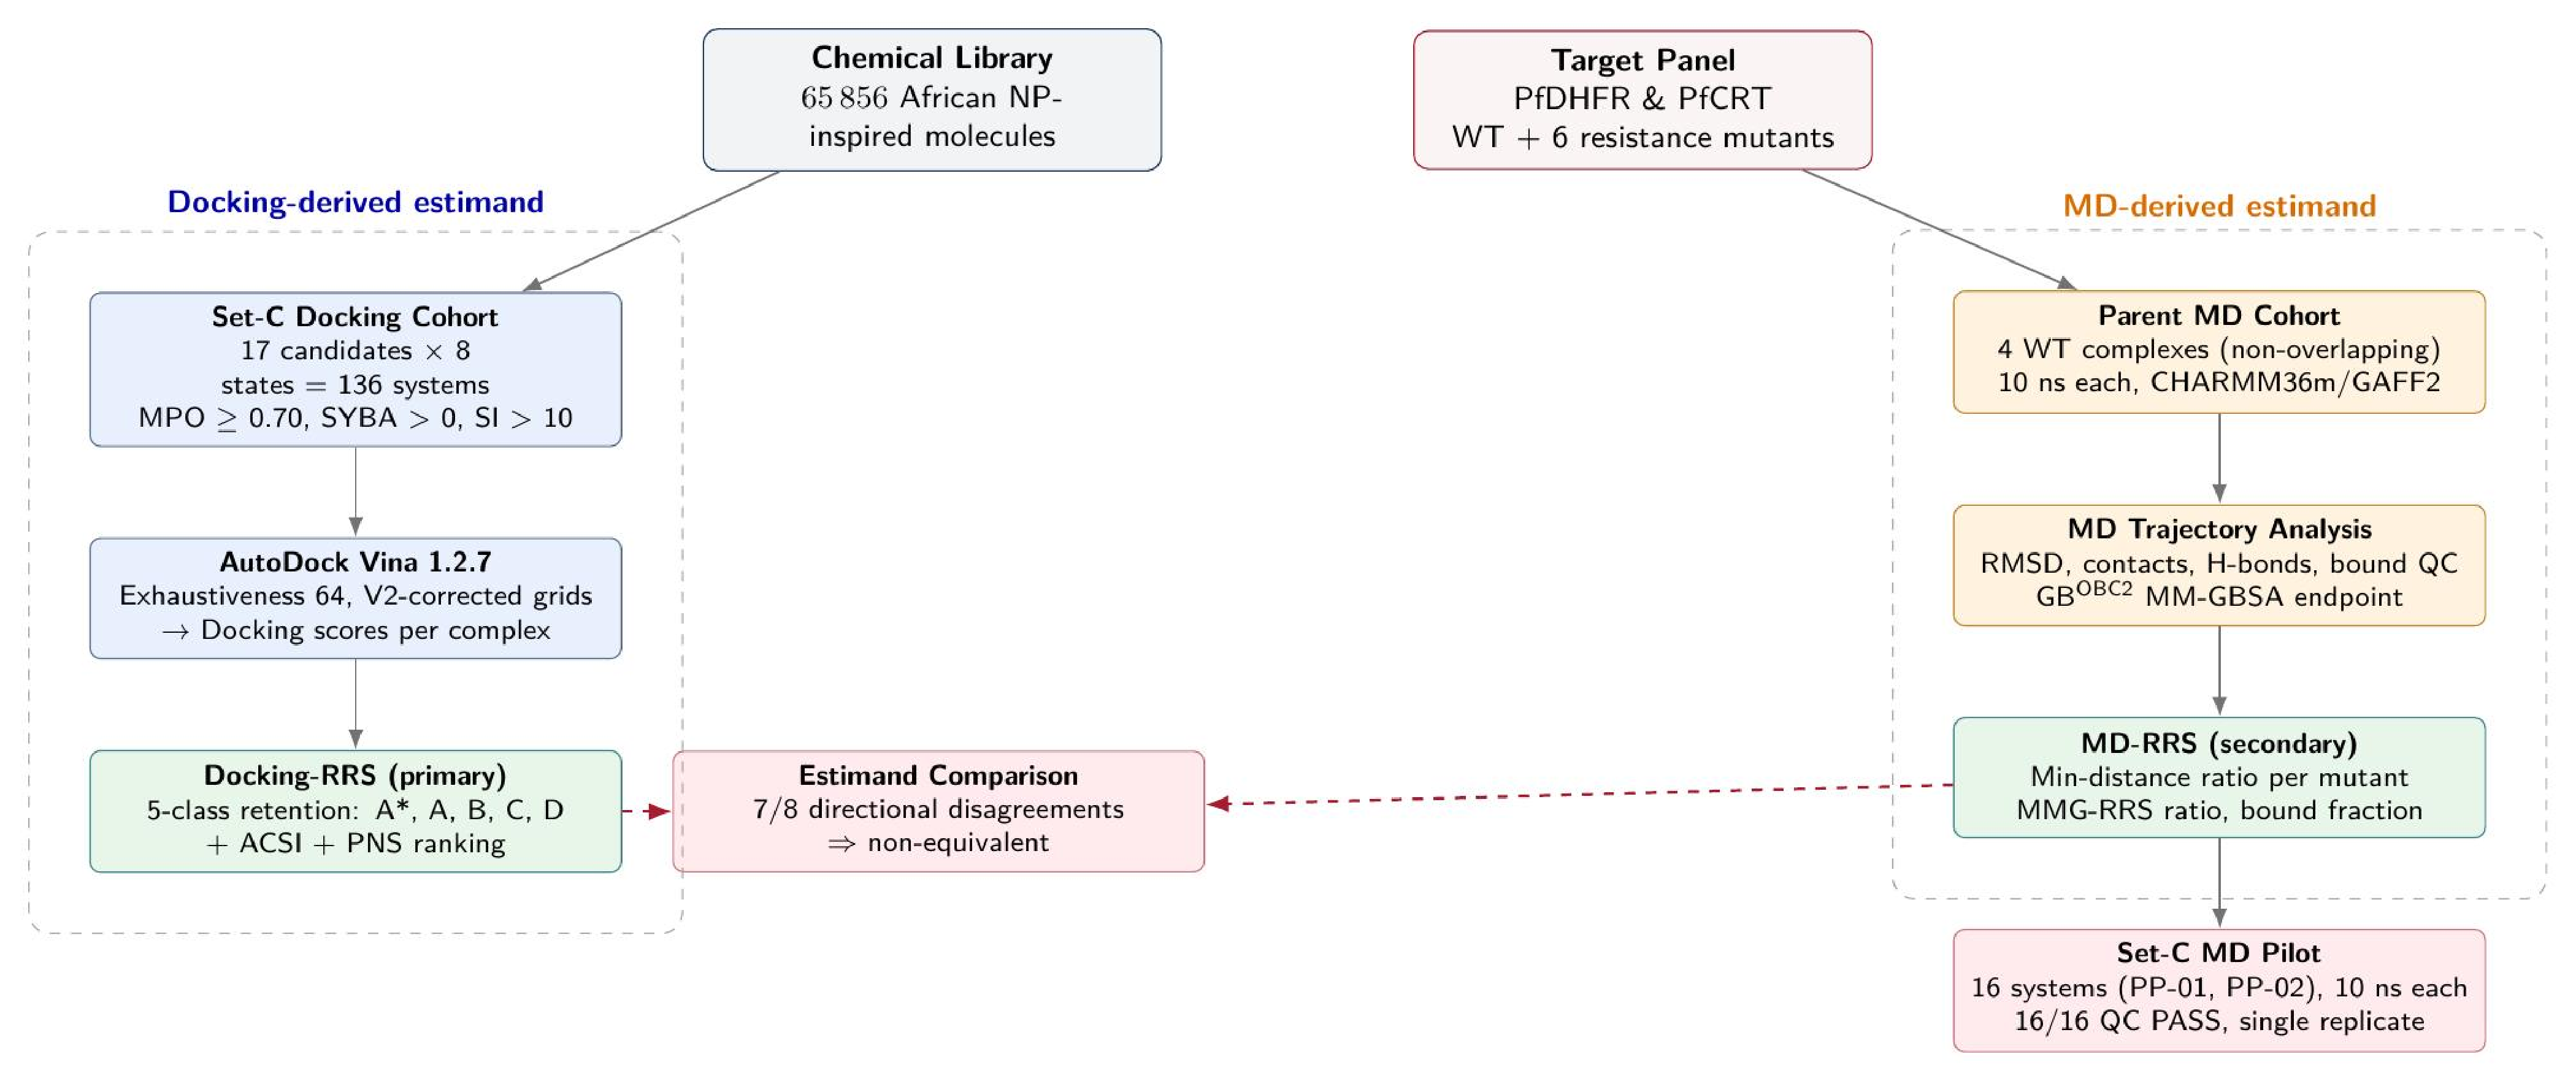
\includegraphics[width=0.98\textwidth]{Graphics/p2_preview-1.pdf}
\caption{\textbf{Integrated Resistance-Aware Polypharmacology and Molecular Dynamics Triage Framework.} Static multi-target docking (PfDHFR, PfCRT, PfATP4, PfClpR) with Resistance-Resilience Scores (RRS), Antimalarial Chemical Space Index (ACSI), and Polypharmacological Network Score (PNS), followed by \qty{10}{\ns} explicit-solvent MD (OpenFF~2.2.0/CHARMM36m) as a secondary check on the protocol-local Estimand Divergence signal (7/8 matched states). \textbf{PP-01} passes the two-target pilot gate; \textbf{PP-02} remains single-target scope and was not promoted; \textbf{PP-15} is a wild-type feasibility probe outside the Set-C estimand with no RRS estimate. Resistance or evolutionary interpretations require prospective experimental validation.}
\label{fig:study_workflow}
\end{figure}

Library provenance and source-class counts follow the upstream library record (Supporting Information Table~S16). Primary candidates were prioritized using multi-parameter optimization (MPO $\ge \num{0.70}$, retaining \num{19913} primary leads), predicted synthetic accessibility (SYBA $> \num{0}$), predicted selectivity index (SI $> \num{10}$), target coverage across at least two docking receptors, and scaffold diversity ($\le 3$ compounds per Bemis--Murcko scaffold). This selection yielded the Set-C candidate panel ($n=\num{17}$). Four additional parent-study production-MD wild-type complexes (systems 201, 214, 438, 164; the 438-labelled system contains upstream index 437) were evaluated; these carry no consensus-lead status and their ligand identities and receptor correspondence are documented in the archived ligand identity review. The 164 system represents PfClpR (PDB 4GM2, not PfClpP). Five approved antimalarial drugs (artemisinin, pyrimethamine, chloroquine, lumefantrine, cipargamin) served as reference controls (\cref{tab:system_breakdown}). Class frequencies are conditional on these filters and should not be extrapolated to the full library.

\begin{table}[htbp]
\centering
\caption{Breakdown of the 136 docking protein--ligand systems by target. The 17 Set-C candidates were docked against 5 PfDHFR states (WT + N51I, C59R, S108N, I164L) and 3 PfCRT states (WT + K76T, K76A).}
\label{tab:system_breakdown}
\small
\begin{tabularx}{\textwidth}{>{\raggedright\arraybackslash}X S[table-format=2.0] S[table-format=1.0] S[table-format=3.0] l}
\toprule
Category & {Ligands} & {Targets} & {Systems} & {MD (\si{\ns})} \\
\midrule
PfDHFR WT + 4 mutants (Set-C) & 17 & 5 & 85 & \textemdash \\
PfCRT WT + 2 mutants (Set-C) & 17 & 3 & 51 & \textemdash \\
\midrule
\textbf{Docking total} & {--} & {--} & \textbf{136} & \textemdash \\
\bottomrule
\multicolumn{5}{p{0.90\textwidth}}{The 136 docking systems were not subjected to production MD. The 16-system pilot and four non-overlapping parent-study complexes were analyzed separately.} \\
\end{tabularx}
\end{table}

\subsection{Resistance mutation panel}

We selected six mutant or comparator states (\cref{tab:mutations}); target identifiers are in the Supporting Information (\cref{SM-tab:s5_plasmodb}). PfDHFR substitutions and PfCRT K76T represent resistance-associated contexts described in WHO resources; K76A is a mechanistic comparator, not a prevalence estimate.

\begin{table}[htbp]
\centering
\caption{Resistance mutation panel.}
\label{tab:mutations}
\begin{tabularx}{\textwidth}{l l l X}
\toprule
Target & State & Resistance context & Evidence boundary \\
\midrule
PfDHFR & N51I & Antifolate-resistance state & Computational panel; no frequency estimate \\
PfDHFR & C59R & Antifolate-resistance state & Computational panel; no frequency estimate \\
PfDHFR & S108N & Antifolate-resistance state & Computational panel; no frequency estimate \\
PfDHFR & I164L & High-level antifolate-resistance state & Comparator for severe resistance \\
PfCRT & K76T & Chloroquine-resistance marker & Transporter-resistance context \\
PfCRT & K76A & Mechanistic comparator for Lys76 perturbation & No clinical prevalence or resistance-marker claim \\
\bottomrule
\end{tabularx}
\end{table}

\subsection{Homology modelling of resistance mutants}

No mutant crystal structures were available for the panel; the six mutant structures were generated with SWISS-MODEL from wild-type templates PfDHFR (7F3Y) and PfCRT (6UKJ). PfATP4 and the 164-labelled parent-MD system were used as deposited crystal structures with no mutants modelled. PDB 4GM2 is PfClpR, not PfClpP. Models were retained only when QMEAN exceeded \num{-4.0}, GMQE exceeded \num{0.7}, Ramachandran favored residues exceeded \qty{95}{\percent}, and backbone RMSD was below \qty{1.5}{\angstrom}. All six models met these thresholds (\cref{SM-tab:s_homology_qc}). Model scores are not experimental structures.

\subsection{Docking protocol assessment}

The docking protocol follows the upstream library workflow (Supporting Information Table~S16): AutoDock Vina 1.2.7~\citep{vina_2021} with exhaustiveness \num{64} against grids centered on the corrected V2 binding-site coordinates~\citep{Temgoua2026} of PfDHFR (7F3Y), PfCRT (6UKJ~\citep{Kim2019PfCRT}), PfATP4 (9N10), and the historically labelled PfClpR/4GM2 entry (not PfClpP). The V2 grid specification represents the post-review refinement from the companion study, including the critical PfCRT K76→LYS restoration for wild-type reference state and P2Rank-validated binding-site centers. P2Rank~\citep{Krivak2018P2Rank} pocket predictions were compared with the grid centers as a boundary audit of these fixed boxes (\cref{SM-fig:s4_p2rank_boxes}).

Parent-study enrichment benchmarks (V2 grids) are summarized here and tabulated in full in the Supporting Information (\cref{SM-tab:s1_docking_validation}). On the MMV Malaria Box consensus (Vina+DiffDock), ROC-AUC was \num{0.924} (PfDHFR), \num{0.971} (PfCRT), and \num{1.000} (PfATP4). In contrast, DEKOIS 2.0 enrichment for PfDHFR with Vina alone was null (ROC-AUC \num{0.450}, $\mathrm{EF}_{5\,\%} = \num{0.00}$), indicating that score-based recovery of known actives is protocol- and library-dependent. Redocking was considered accurate when heavy-atom RMSD was $<$ \qty{2.0}{\angstrom} relative to the crystal pose; the MTX redock attempt was a clear failure (RMSD $\approx$ \qty{30}{\angstrom}). AutoDock Vina was used for all reported Set-C scores; GNINA pose scoring yielded no usable score for the Set-C panel (the secondary 39-compound panel below uses GNINA CNN affinity rescoring). Docking scores are empirical scoring approximations that are sensitive to the scoring function and protocol~\citep{ferreira2023docking,sadybekov2023computational,kittelson2026docking}; they should not be treated as binding free energies.

\subsection{Secondary docking calibration}

A secondary Tartarus cross-docking analysis used QuickVina on the primary-lead panel. The composite MPO--docking-score association was null in this exploratory check; complete correlations are provided in the Supporting Information (\cref{SM-tab:secondary_tartarus_calibration,SM-tab:secondary_tartarus_correlation}).

\subsection{Retrospective confrontation with published genotype--phenotype data}

As an external, purely retrospective check of the static $\Delta\Delta G$ estimand, we curated IC$_{50}$ records for \textit{Pf}DHFR (ChEMBL target CHEMBL1939~\citep{zdrazil2024chembl}) by assay description, which encodes the DHFR genotype. The curated set contains 28 compounds with paired wild-type and quadruple-mutant (N51I/C59R/S108N/I164L) measurements; 24 of them also carry paired double-mutant (C59R/S108N) measurements, and triple-mutant (C59R/S108N/I164L) pairs are complete for all 28. Assay identifiers, raw records, and provenance are frozen with the analysis and described in Data Availability. These are whole-parasite growth IC$_{50}$ values from DHFR-genotyped strains with distinct genetic backgrounds (wild-type TM4/8.2, double-mutant K1CB1, triple-mutant Csl-2, quadruple-mutant Vl/S), not isogenic recombinant-enzyme measurements. We therefore use them descriptively as a phenotype-level reference, not as a binding-affinity ground truth. This genotype-resolved curation differs from the upstream activity-transfer panel audited in the Supporting Information (\cref{SM-tab:s15_robustness_transfer}), which carries compound-level activity labels without genotype pairing.

The 28 compounds were docked against the wild-type, double, triple, and quadruple \textit{Pf}DHFR states with the declared Vina protocol (AutoDock Vina 1.2.7, exhaustiveness \num{64}, fixed V2 \textit{Pf}DHFR box, single seed \num{42}; \num{112}/\num{112} jobs completed). Double, triple, and quadruple receptors were generated from the wild-type coordinates by in silico side-chain replacement with backbone coordinates unchanged, then prepared identically under the same protocol. For each genotype, $\Delta\Delta G = s_{\mathrm{mutant}} - s_{\mathrm{WT}}$ was compared with the published fold-shift $\log_2(\mathrm{IC}_{50,\mathrm{mut}}/\mathrm{IC}_{50,\mathrm{WT}})$ using Spearman rank correlation, direction agreement (both quantities positive or both negative), and an exact binomial probability of the observed departure from chance agreement (\cref{SM-tab:s20_chembl_foldshift}).

\subsection{African Natural Product chemical space and structural descriptors}

The candidate panel (Set-C, $n=\num{17}$) was derived from the African Natural Products Database (ANPDB) and synthetic antimalarial reference sets. Physicochemical and stereochemical descriptors were computed using RDKit (v2025.03.6). The cohort exhibits a mean molecular weight ($\mathrm{MW}$) of \qty{271.9 \pm 69.3}{\g\per\mole}, a partition coefficient ($\mathrm{LogP}$) of \num{2.84 \pm 0.82}, a quantitative estimate of drug-likeness ($\mathrm{QED}$) of \num{0.70 \pm 0.06}, a fraction of $sp^3$-hybridized carbons ($Fsp^3$) of \num{0.22 \pm 0.15}, and an average of \num{0.6 \pm 0.9} chiral centers per molecule.

These properties reflect compact, low-molecular-weight natural product cores (including prenylated chromones, flavonoid derivatives, and indole alkaloids) isolated from African medicinal flora such as \textit{Cryptolepis sanguinolenta}, \textit{Enantia chlorantha}, and \textit{Artemisia} species. The high mean MPO score (\num{0.728 \pm 0.021}) and synthetic accessibility scores ($\mathrm{SYBA} = \num{36.6 \pm 23.4}$) indicate chemical-space alignment with synthetic feasibility.

\subsection{MPO sensitivity and predicted ADMET profile}

MPO-weight sensitivity and single-source ADMET-AI predictions were used descriptively; the complete sensitivity and endpoint results are provided in the Supporting Information (\cref{SM-fig:s1_mpo_sensitivity,SM-tab:s3_admet}). These predictions were not experimentally validated.

\subsection{Docking-derived resistance-retention score definition}\label{sec:rrs_formula}

All 17 candidates were docked against each wild-type and mutant structure using AutoDock Vina 1.2.7 with exhaustiveness \num{64}. The 136 systems were ranked with empirical Vina scores rather than calibrated binding free energies. Grid boxes were centered on the co-crystallized ligand position with \qty{25}{\angstrom} dimensions, matching the audited V2 configuration files~\citep{Temgoua2026}.

For target $t$, let $s_{\mathrm{Vina},i,\mathrm{WT},t}$ and $s_{\mathrm{Vina},i,m,t}$ denote the signed Vina scores. Candidates with $|s_{\mathrm{Vina},i,\mathrm{WT},t}| < \qty{5.0}{\kcalmol}$ are excluded from that target's score-retention analysis. The target-specific resistance-retention score (RRS) is
\begin{equation}
\mathrm{RRS}_{i,m,t} = \frac{|s_{\mathrm{Vina},i,m,t}|}{|s_{\mathrm{Vina},i,\mathrm{WT},t}|} \times 100.
\end{equation}
RRS is a relative docking-score-retention statistic, not a free-energy difference or resistance measurement. The available-target summary averages the defined target-specific values across eligible targets and mutant states. The primary analysis is restricted to the 12 candidates with eligible PfDHFR and PfCRT wild-type scores; the five PfCRT-only candidates are reported separately.

The mutually exclusive classes are defined from the available mutant values; primary class counts use the complete two-target subset:
\begin{itemize}
    \item \textbf{Class A*}: all available mutant RRS values are at least \qty{80}{\percent} and the minimum eligible wild-type score magnitude is at least \qty{7.0}{\kcalmol}.
    \item \textbf{Class A}: all available mutant RRS values are at least \qty{80}{\percent}, but the minimum eligible wild-type score magnitude is below \qty{7.0}{\kcalmol}.
    \item \textbf{Class B}: all available mutant RRS values are at least \qty{70}{\percent}, but at least one is below \qty{80}{\percent}.
    \item \textbf{Class C}: at least one available mutant RRS value is at least \qty{80}{\percent}, but not all available values reach \qty{70}{\percent}.
    \item \textbf{Class D}: no available mutant RRS value reaches \qty{80}{\percent}.
\end{itemize}
The classes are mutually exclusive. The cut-offs follow the Vina score distribution in this panel and are not calibrated to biochemical resistance or clinical outcome. Sensitivity to alternative thresholds is in the Supporting Information (\cref{SM-tab:s11_rrs_threshold_sensitivity}).

\subsection{Secondary ranking descriptors}

ACSI places each candidate relative to approved-drug and African natural-product reference spaces; weight-sensitivity checks are in the Supporting Information (\cref{SM-tab:s4_acsi_sensitivity}). PNS is a network-weighted ranking score; PfCRT centrality was imputed, with sensitivity reported in the Supporting Information (\cref{SM-tab:s7_pns_sensitivity}). Associations among metrics were assessed by Spearman rank correlation with \num{100000} permutations, Bonferroni adjustment for three tests, and bootstrap intervals from \num{10000} resamples. At $n=\num{12}$ these correlations are descriptive and are not powered tests of independence.

\subsection{MD protocol}

We simulated all four parent-study wild-type systems for \qty{10}{\ns} with CHARMM36m~\citep{charmm36m_2017}/GAFF2~\citep{wang2004gaff} at \qty{310.15}{\kelvin} using GROMACS~\citep{gromacs_2015,lindahl_2024}. The \qty{10}{\ns} length is intended as a pose-retention and local-geometry check, not as a measurement of residence time or converged free energy~\citep{wei2024structure}. We analyzed the trajectories after removing periodic-boundary discontinuities. MDAnalysis~\citep{mdanalysis_2011} was used to calculate contacts, H-bonds, RMSF, and radius of gyration every \num{10} frames and RMSD on every frame.

We obtained MM-GBSA endpoint estimates from production trajectories using the GB$^{\text{OBC2}}$ model (igb=5) with \qty{0.15}{\molar} salt, via the \texttt{gmx\_MMPBSA} v1.5.0.3~\citep{gmx_mmpbsa_2021} CHARMM36-to-AMBER conversion. These are endpoint enthalpic scores, not rigorous free energies, and their limits for ranking dissimilar complexes are well documented~\citep{roux2024mmgbsa}. Predicting mutation effects with endpoint methods remains hard, with best-case correlations near 0.44 even at \qty{100}{\ns}~\citep{yu2022mutation_mmgbsa}. We did not include configurational entropy. For the interpretable parent-study and PP-15 summaries we report frame-level SEM; the Set-C table instead shows the propagated within-trajectory standard deviation (SD$_{\mathrm{prop}}$). Neither quantity is a replicate-level uncertainty estimate. The inter-replicate diagnostic is reported separately in the Supporting Information.

The 16-system Set-C pilot used the same temperature and length, with ligand parameters from OpenFF 2.2.0 (AM1-BCC) rather than GAFF2. Absolute MM-GBSA values are therefore not compared between the two cohorts. Each mutant was run as a single replicate; trajectories were accepted for endpoint analysis only after geometric quality checks. Trajectory-based retention is summarized as $\mathrm{MD\text{-}RRS}_{\mathrm{distance}} = \num{100} \times \langle d_{\min} \rangle_{\mathrm{mut}} / \langle d_{\min} \rangle_{\mathrm{WT}}$, where $d_{\min}$ is the minimum heavy-atom protein--ligand distance; values at or below \qty{100}{\percent} indicate pose retention at least as tight as the wild-type endpoint, not increased affinity.

% ============================================================================
% 3. RESULTS
% ============================================================================

\section{Results}

\subsection{Operational reproducibility of the docking-RRS signal}

Mean target-specific RRS was 75.1 for PfDHFR (12 candidates) and 86.2 for PfCRT (17 candidates); full target-wise summaries are in the Supporting Information (\cref{SM-tab:s12_rrs_by_target}). The difference reflects docking-score retention between panels, not biological resistance.

On the complete two-target set ($n=\num{12}$) the classes were A*:~\num{1}, A:~\num{1}, B:~\num{4}, C:~\num{5}, and D:~\num{1}. On all 17 candidates classified on eligible targets, the counts become A*:~\num{5}, A:~\num{1}, B:~\num{5}, C:~\num{5}, and D:~\num{1}. The five PfCRT-only compounds are not comparable with the two-target set. Per-compound RRS profiles are shown in \cref{SM-fig:s2_rrs_radar}. Varying the wild-type eligibility threshold from \qty{4.0}{\kcalmol} to \qty{5.0}{\kcalmol} left class counts unchanged. Raising retention thresholds from \qty{70}{\percent}/\qty{80}{\percent} to \qty{80}{\percent}/\qty{90}{\percent} increased Class~D from 1 to 9 (\cref{SM-tab:s11_rrs_threshold_sensitivity}).

The docking-RRS signal is reproducible under the declared protocol: PP-01 multi-seed dispersion is $\pm\qty{0.05}{\kcalmol}$ for PfDHFR and $\pm\qty{0.04}{\kcalmol}$ for PfCRT, and PP-15 multi-seed dispersion is $\pm\qty{0.03}{\kcalmol}$. In a bounded score-perturbation audit, \qty{77.9}{\percent} of RRS classes remained unchanged under $\pm\qty{1}{\kcalmol}$ perturbation. This characterizes protocol-level consistency, not pose accuracy or binding fidelity.

\subsection{Chemical-space and network descriptors (secondary)}

The mean ACSI for the 17-candidate cohort was \num{0.543}, with two candidates (\qty{11.8}{\percent}) exceeding \num{0.70} on the approved-drug/African-NP reference space; weight-sensitivity checks are in the Supporting Information (\cref{SM-tab:s4_acsi_sensitivity}). PNS was only weakly associated with RRS on the two-target set ($\rho=\num{-0.2098}$, adjusted $p=\num{1.0000}$); PfCRT centrality was imputed, with sensitivity reported in the Supporting Information (\cref{SM-tab:s7_pns_sensitivity}). At $n=\num{12}$ the wide bootstrap intervals are consistent with distinct rather than redundant ranking dimensions, but they are too wide to establish independence.

\subsection{Cross-metric associations (secondary, post-selection)}

These secondary, post-selection comparisons test whether docking-derived RRS aligns with PNS and ACSI within the same cohort; they are not independent validation of any mechanism.

\begin{figure}[htbp]
\centering
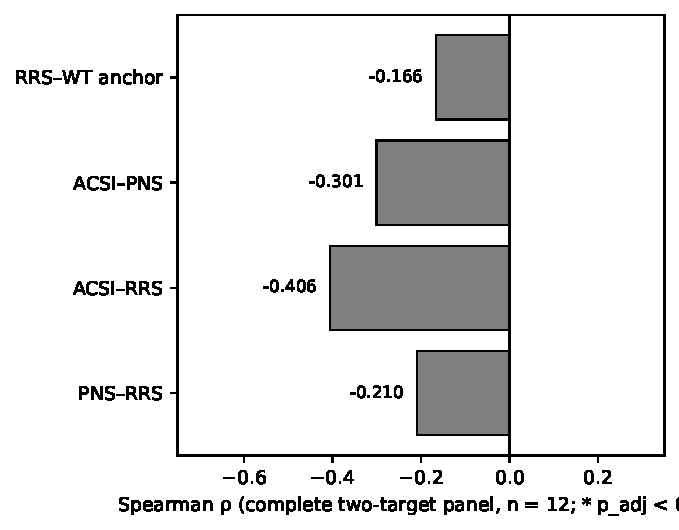
\includegraphics[width=0.85\textwidth]{Graphics/cross_metric_correlation.pdf}
\caption{\textbf{Cross-metric Spearman correlations.} Complete two-target panel ($n=\num{12}$): PNS--RRS $\rho=-\num{0.2098}$, ACSI--RRS $\rho=-\num{0.4056}$, ACSI--PNS $\rho=-\num{0.3007}$, RRS--weakest-WT-anchor $\rho=-\num{0.1661}$; none significant after Bonferroni correction ($p_{\mathrm{adj}} \geq \num{0.51}$; \num{100000} permutations, seed \num{42}). Values from the cross-metric statistical audit.}
\label{fig:crossmetric}
\end{figure}

\begin{table}[htbp]
\centering
\caption{Cross-metric Spearman correlations on the complete two-target set ($n=\num{12}$). Permutation $p$-values use \num{100000} permutations; adjusted $p$-values use Bonferroni correction for three tests. Bootstrap intervals are percentile \qty{95}{\percent} intervals from \num{10000} resamples.}
\label{tab:crossmetric}
\small
\begin{tabular}{@{}l S[table-format=-1.4] S[table-format=1.4] S[table-format=1.4] l@{}}
\toprule
Metric pair & {Spearman $\rho$} & {$p_{\mathrm{perm}}$} & {$p_{\mathrm{adj}}$} & {Bootstrap 95\% CI} \\
\midrule
PNS vs.\ RRS & -0.2098 & 0.5144 & 1.0000 & $[-0.76,\,0.54]$ \\
ACSI vs.\ RRS & -0.4056 & 0.1922 & 0.5766 & $[-0.89,\,0.29]$ \\
RRS vs.\ weakest WT score & -0.1661 & 0.6038 & 1.0000 & $[-0.73,\,0.59]$ \\
\bottomrule
\end{tabular}
\end{table}

On the two-target set ($n=\num{12}$), all three correlation coefficients were non-significant after Bonferroni correction: PNS--RRS $\rho=\num{-0.2098}$, ACSI--RRS $\rho=\num{-0.4056}$, RRS--weakest WT score $\rho=\num{-0.1661}$ (\cref{tab:crossmetric}). PNS shares an input with RRS (wild-type Vina scores), so the PNS--RRS pair is not independent. On all 17 candidates, PNS--RRS strengthened ($\rho=-0.5588$, adjusted $p=0.0667$). Unequal target coverage limits interpretation there.

\subsection{Computational prioritization intersection (exploratory)}

Requiring Class~A or A*, ACSI $>$ \num{0.5}, and above-mean PNS leaves one candidate on the two-target panel. That intersection is reported as a shortlist for experiment, not as evidence of activity or resistance resilience.

\subsection{Parent-study MD check (non-overlapping cohort, secondary)}

Four non-overlapping parent-study wild-type complexes were simulated for \qty{10}{\ns} as a secondary pose-retention check; these compounds are not among the 17 Set-C candidates and do not validate the Set-C ranking.

\begin{table}[htbp]
\centering
\caption[MD stability metrics]{Production MD stability metrics for parent-study wild-type complexes (\qty{10}{\ns}). BB RMSD, ligand RMSD, minimum distance, contacts, and H-bonds are computed from PBC-unwrapped trajectories.}
\label{tab:md_stability}
\resizebox{\textwidth}{!}{%
\begin{tabular}{@{}l c S[table-format=2.2] S[table-format=2.2] S[table-format=2.2] S[table-format=3.1] S[table-format=2.1] l@{}}
\toprule
Target & {Atoms} & {BB RMSD (\si{\angstrom})} & {Lig. RMSD (\si{\angstrom})} & {Min dist (\si{\angstrom})} & {Contacts} & {H-bonds} & Interpretation \\
\midrule
PfClpR-labelled cohort (system 164)   & \num{43035}  & 1.31 & 1.11 & 67.42 & 0.0   & 23.7 & Unbound \\
PfDHFR (system 201)   & \num{134153} & 3.05 & 1.70 & 78.21 & 0.0   & 21.5 & Unbound \\
PfCRT (system 214)    & \num{76920}  & 4.47 & 2.45 & 3.19  & 78.1  & 23.1 & Bound \\
PfATP4 (system 438)   & \num{420801} & 12.27& 2.13 & 2.25  & 178.4 & 47.7 & Bound \\
\bottomrule
\end{tabular}%
}
\end{table}

\begin{figure}[htbp]
\centering
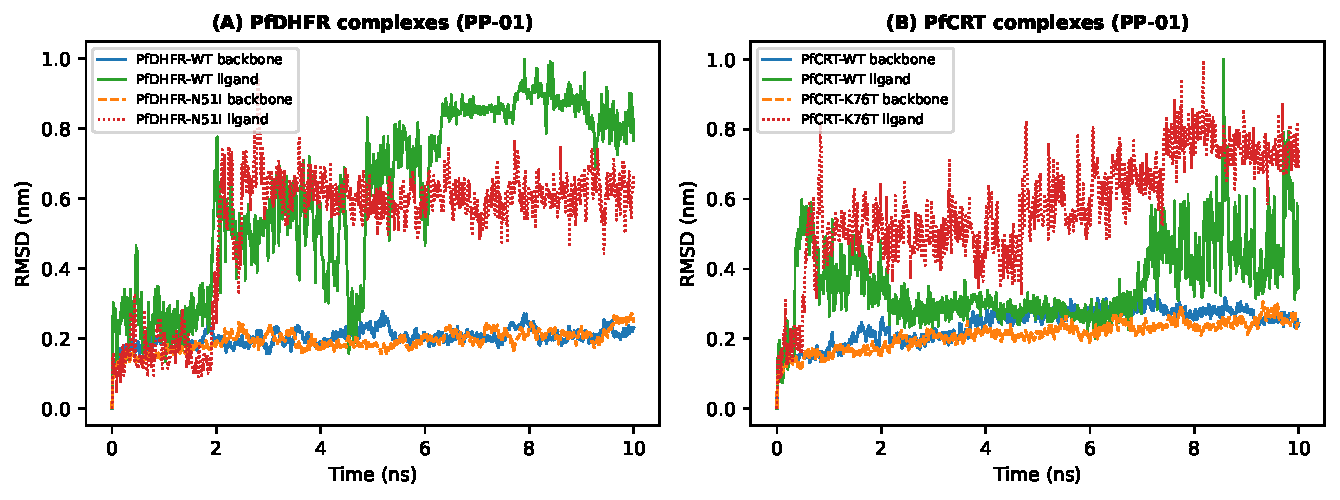
\includegraphics[width=\textwidth]{Graphics/Figure3_RMSD_Stability.pdf}
\caption{\textbf{Pose retention and thermal equilibration (canonical R1 trajectories).} Explicit-solvent backbone (solid) and ligand-after-backbone-fit (dashed/dotted) RMSD time-series (\qty{10}{\ns}) for \textbf{PP-01}, computed with \texttt{gmx rms} (PBC-whole reconstruction; fit group = Backbone; RMS groups = Backbone / MOL\num{0}). (A) \textit{Pf}DHFR: backbone \qty{0.203 \pm 0.024}{\nm} (WT), \qty{0.193 \pm 0.029}{\nm} (N51I); ligand \qty{0.613 \pm 0.240}{\nm} and \qty{0.519 \pm 0.190}{\nm}. (B) \textit{Pf}CRT: backbone \qty{0.241 \pm 0.048}{\nm} (WT), \qty{0.211 \pm 0.039}{\nm} (K76T); ligand \qty{0.357 \pm 0.113}{\nm} and \qty{0.581 \pm 0.155}{\nm}. All trajectories pass the geometric QC gate (mean minimum heavy-atom distance \numrange{2.7}{3.2}\,\si{\angstrom}, bound fraction \num{1.000}); ligand RMSD reflects in-pocket mobility, not dissociation.}
\label{fig:rmsd_stability}
\end{figure}

\begin{table}[htbp]
\centering
\caption[Parent-study MM-GBSA interpretation]{Endpoint energy evaluation for four reference wild-type complexes. Only the PfCRT complex yields an interpretable MM-GBSA endpoint; dissociated systems and conversion anomalies are N/A.}
\label{tab:mmgbsa}
\small
\begin{tabularx}{\textwidth}{@{}l l S[table-format=-2.2] S[table-format=1.2] >{\raggedright\arraybackslash}X@{}}
\toprule
System & Target & {$\Delta G_{\mathrm{bind}}$ (\si{\kcalmol})} & {SEM} & Interpretation \\
\midrule
System 214 & PfCRT-WT & -18.25 & 0.40 & Stable anchorage; ligand bound$^\dagger$ \\
System 164 & PfClpR-WT & {--} & {--} & N/A; ligand dissociated$^\ddagger$ \\
System 201 & PfDHFR-WT & {--} & {--} & N/A; ligand dissociated$^\S$ \\
System 438 & PfATP4-WT & {--} & {--} & N/A; parameter conversion anomaly$^\ast$ \\
\bottomrule
\multicolumn{5}{p{0.95\textwidth}}{$^\dagger$Ligand remains bound (minimum distance \qty{3.19}{\angstrom}, \num{78} contacts); calculated via \texttt{gmx\_MMPBSA}. Uncertainty is the SEM over \num{101} stored snapshots.} \\
\multicolumn{5}{p{0.95\textwidth}}{$^\ddagger$Ligand separates beyond \qty{60}{\angstrom} minimum distance with zero contact persistence; excluded from binding energy evaluation.} \\
\multicolumn{5}{p{0.95\textwidth}}{$^\S$As $^\ddagger$ (PfDHFR system).} \\
\multicolumn{5}{p{0.95\textwidth}}{$^\ast$Excluded: multi-chain membrane-transporter parameterization introduced force-field conversion artifacts.} \\
\end{tabularx}
\end{table}

Of the four reference complexes, two retained stable protein--ligand contacts while two dissociated (\cref{tab:md_stability}); for PfATP4, force-field parameter conversion precluded reliable MM-GBSA endpoints (\cref{tab:mmgbsa}).



\subsection{Estimand Divergence Between Static Docking and Dynamic Trajectories}

The primary docking retention metrics and trajectory-based geometric stability summaries are non-equivalent computational estimands. Explicit-solvent MD was run on PP-01 and PP-02 across 16 receptor states; all 16 trajectories satisfied geometric contact stability thresholds (\qty{<3.5}{\angstrom} minimum protein--ligand distance).

For the eight mutant states with an eligible wild-type docking baseline, static grid docking predicted reduced score retention ($RRS < \qty{100}{\percent}$). Explicit-solvent relaxation pointed the other way in \qty{87.5}{\percent} (7/8; 95\% Wilson CI \qtyrange{52.9}{97.8}{\percent}, $n=\num{8}$) of matched comparisons ($\mathrm{MD\text{-}RRS}_{\mathrm{distance}} \le \qty{100}{\percent}$). The interval excludes the \qty{50}{\percent} chance level, though it is wide at $n=\num{8}$. At single-replicate scope this mismatch is an observed calibration signal, not a demonstrated mechanism. Static docking scores ($\Delta G_{\mathrm{grid}}$) and trajectory-derived retention ratios ($\mathrm{MD\text{-}RRS}_{\mathrm{distance}}$) are complementary triage signals, not interchangeable measures of binding free energy.

We ran a single-ligand feasibility probe (\textbf{PP-15}, outside the 16-system Set-C MD array and the Set-C RRS estimand) on wild-type \textit{Pf}DHFR (7F3Y) and \textit{Pf}CRT (6UKJ). Both systems completed \qty{10}{\ns} production trajectories with \qty{100}{\percent} QC-PASS status (\text{bound fraction} = \num{1.000}). Mean minimum heavy-atom distances were \qty{2.77}{\angstrom} (\textit{Pf}DHFR) and \qty{3.20}{\angstrom} (\textit{Pf}CRT); MM-GBSA endpoints were \qty{-29.52 \pm 0.33}{\kcalmol} (\textit{Pf}DHFR) and \qty{-27.79 \pm 0.49}{\kcalmol} (\textit{Pf}CRT; \cref{SM-tab:s_pp15}). Multi-seed redocking confirmed docking score stability ($\pm\qty{0.03}{\kcalmol}$; \cref{SM-tab:s17_multiseed_redock}). We report no mutant or RRS estimate for this probe and make no dual-target resilience claim from it.

\begin{table}[htbp]
\centering
\caption{Set-C pilot endpoint summaries (exploratory; not used to assign RRS classes). $\Delta G_{\mathrm{bind}}$ is the mean over \num{100} snapshots $\pm$ SD$_{\mathrm{prop}}$ (within-trajectory SD, not SEM or replicate-level uncertainty). The PP-01 PfCRT K76A endpoint (\qty{-35.29}{\kcalmol}) carries a \qty{7.75}{\kcalmol} inter-replicate sensitivity (second trajectory \qty{-27.54}{\kcalmol}; \cref{SM-tab:s19_k76a_replicate}) and supports no resilience claim. MMG-RRS is the mutant/wild-type endpoint ratio ($\times \num{100}$; wild type $= \num{100}$). Docking RRS is shown for comparison (n/a: no wild-type docking reference for PP-02 PfDHFR). Single-replicate summaries are within-protocol contrasts only.}\label{tab:mmgbsa_setc}
\scriptsize
\begin{tabular}{@{}l l l S[table-format=-2.2] S[table-format=1.2] S[table-format=3.1] S[table-format=3.2]@{}}
\toprule
Candidate & Target & State & {$\Delta G_{\mathrm{bind}}$ (\si{\kcalmol})} & {SD$_{\mathrm{prop}}$} & {MMG-RRS} & {Docking RRS} \\
\midrule
PP-01 & PfCRT & K76A & -35.29 & 1.17 & 115.3 & 90.86 \\
PP-01 & PfCRT & K76T & -29.51 & 2.65 & 96.4 & 92.47 \\
PP-01 & PfCRT & WT & -30.61 & 1.65 & 100.0 & {--} \\
PP-01 & PfDHFR & C59R & -26.56 & 1.91 & 105.0 & 85.47 \\
PP-01 & PfDHFR & I164L & -26.13 & 2.34 & 103.3 & 83.87 \\
PP-01 & PfDHFR & N51I & -29.83 & 1.50 & 118.0 & 86.40 \\
PP-01 & PfDHFR & S108N & -30.21 & 3.62 & 119.5 & 87.60 \\
PP-01 & PfDHFR & WT & -25.29 & 2.94 & 100.0 & {--} \\
PP-02 & PfCRT & K76A & -24.53 & 1.27 & 97.8 & 94.62 \\
PP-02 & PfCRT & K76T & -30.45 & 1.38 & 121.4 & 87.91 \\
PP-02 & PfCRT & WT & -25.08 & 2.56 & 100.0 & {--} \\
PP-02 & PfDHFR & C59R & -28.85 & 1.88 & 95.7 & n/a \\
PP-02 & PfDHFR & I164L & -31.06 & 1.52 & 103.0 & n/a \\
PP-02 & PfDHFR & N51I & -34.02 & 2.68 & 112.8 & n/a \\
PP-02 & PfDHFR & S108N & -27.09 & 1.55 & 89.8 & n/a \\
PP-02 & PfDHFR & WT & -30.16 & 2.06 & 100.0 & {--} \\
\bottomrule
\end{tabular}
\end{table}

\subsection{Additional docking sensitivity panel}

The 39-ligand docking sensitivity panel produced \num{312} finite docking scores across the same eight PfDHFR/PfCRT states. Bootstrap mean RRS was \num{100.45} (\numrange{99.59}{101.32}) and the Class-A fraction was \num{0.974} (\numrange{0.923}{1.000}). A mean near \num{100} means that mutant and wild-type Vina scores were on average nearly proportional under this protocol. This is a computational sensitivity check, not validation of the Set-C ranking or of experimental resistance (\cref{SM-tab:s15_robustness_transfer}).

\subsection{Retrospective comparison against published \textit{Pf}DHFR fold-shifts}

The curated ChEMBL panel asked directly whether static $\Delta\Delta G$ reproduces published genotype-level resistance shifts (\cref{SM-tab:s20_chembl_foldshift}). It did not. Spearman $\rho$ between $\Delta\Delta G$ and the $\log_2$ fold-shift was \num{0.19} ($p=\num{0.375}$, $n=\num{24}$) for the double mutant, $-\num{0.04}$ ($p=\num{0.853}$, $n=\num{28}$) for the triple mutant, and $-\num{0.13}$ ($p=\num{0.504}$, $n=\num{28}$) for the quadruple mutant. Direction agreement was \num{10}/\num{24} (\qty{41.7}{\percent}), \num{9}/\num{28} (\qty{32.1}{\percent}), and \num{8}/\num{28} (\qty{28.6}{\percent}), respectively; for the triple and quadruple mutants the rate departs from chance toward disagreement (exact binomial $p=\num{0.044}$ and $p=\num{0.018}$; double $p=\num{0.271}$). These three per-genotype tests are unadjusted: Bonferroni correction gives \num{0.132} and \num{0.054} for the triple and quadruple mutants, so we report the rates as descriptive evidence of below-chance agreement rather than formal rejections. Reference DHFR inhibitors pyrimethamine (\num{919}-fold) and cycloguanil (\num{145}-fold) were mispredicted directionally at every genotype. Mutant scores averaged slightly more favorable than wild-type scores (mean $\Delta\Delta G$ \qtyrange{-0.19}{-0.12}{\kcalmol} across genotypes; \qtyrange{68}{79}{\percent} of compounds below zero), a systematic shift smaller than the $\pm\qty{1}{\kcalmol}$ score sensitivity of the protocol. Given the phenotype-level, non-isogenic reference, this comparison stays descriptive: it tests the static $\Delta\Delta G$ estimand against published measurements, not the Set-C candidates.

% ============================================================================
% 4. DISCUSSION
% ============================================================================

\section{Discussion}

\subsection{Resistance-Resilience Stratification and Protocol Robustness}

The Resistance-Resilience Score (RRS) stratifies the primary candidate cohort ($n=\num{12}$) into five tiers (A*--D) decoupling wild-type binding strength from mutant-state score retention. Under the declared protocol, multi-seed dispersion remained within $\pm\qty{0.05}{\kcalmol}$ (PP-01 and PP-15 across PfDHFR and PfCRT), and \qty{77.9}{\percent} of class assignments were invariant to $\pm\qty{1.0}{\kcalmol}$ score perturbations.

Protocol robustness was tested on an external 39-compound sensitivity panel (\num{312} docking complexes; \cref{SM-tab:s15_robustness_transfer}). GNINA CNN cross-scoring showed \qty{100}{\percent} class-level agreement with Vina, with no per-mutant rank transfer claimed (per-mutant $\rho$ near zero for C59R/I164L). Because almost the whole panel falls in Class A (bootstrap Class-A fraction \num{0.974}), this agreement is close to degenerate and constrains only gross class assignment, not ranking quality. On the DEKOIS 2.0 PfDHFR benchmark, Vina ROC-AUC was \num{0.450} ($\mathrm{EF}_{5\,\%} = \num{0.00}$) — chance level, cautioning against treating RRS as a calibrated predictor outside the primary cohort; MD is reported as a parallel structural check, not a validation of docking classes.

Our candidates originate from African natural-product chemical space, without claiming ethnobotanical validation. The panel's drug-likeness ($\mathrm{QED} = \num{0.70 \pm 0.06}$) and synthetic accessibility ($\mathrm{SYBA} = \num{36.6 \pm 23.4}$) are consistent with actionable synthetic feasibility; confirmation requires prospective experiment.

A retrospective confrontation with published genotype-resolved \textit{Pf}DHFR fold-shifts (ChEMBL, 28 paired compounds) reached the same conclusion from experimental data: static $\Delta\Delta G$ did not track whole-parasite resistance shifts at any genotype ($\rho$ \numrange{-0.13}{0.19}, direction agreement \qtyrange{28.6}{41.7}{\percent}). This matches the chance-level DEKOIS enrichment above and the estimand-divergence framing: a single rigid-grid score difference does not estimate phenotype-level resistance. The comparison neither validates nor invalidates the RRS tiers of the primary cohort. RRS is a within-protocol score-retention statistic on anchored poses for the disjoint Set-C compounds; the ChEMBL endpoint is whole-parasite growth in non-isogenic backgrounds, where permeability, efflux, and background mutations contribute. The two analyses address different estimands (\cref{SM-tab:s20_chembl_foldshift}). We performed no experimental measurement on the Set-C candidates themselves; prospective validation remains the outstanding anchor (see Limitations).

\subsection{Estimand Divergence as a Structural Stress-Testing Filter}

We report \textit{Estimand Divergence} between static docking RRS and short explicit-solvent MD pose retention ($\mathrm{MD\text{-}RRS}_{\mathrm{distance}}$) as a protocol-local observation. In \qty{87.5}{\percent} (7/8; 95\% Wilson CI \qtyrange{52.9}{97.8}{\percent}, $n=\num{8}$) of matched mutant states, grid docking predicted score penalties ($RRS < \qty{100}{\percent}$) while MD retained poses ($\mathrm{MD\text{-}RRS}_{\mathrm{distance}} \le \qty{100}{\percent}$); the Wilson interval excludes the \qty{50}{\percent} chance level.

Rigid grid docking evaluates unrelaxed steric complementarity ($\Delta G_{\mathrm{grid}}$), whereas short MD captures local conformational adaptation, hydrogen-bond rearrangement, and solvent-shielded stabilization. Per the JCIM MD reporting guidelines~\citep{soares2023mdreport}, the \qty{10}{\ns} trajectories are secondary structural checks, consistent with established MD-based pose-stability filtering of docked poses~\citep{liu2017mdfilter} but applied here to resistance-mutant triage rather than pose selection. A thermal noise floor of \qty{2.01}{\kcalmol} from independent WT replicates (PP-01 PfCRT WT R1/R2) bounds numerical variation of end-state estimates at this scope. Contemporaneous docking-plus-MD surveys of resistance mutants report qualitative structural conclusions without quantifying this concordance \citep{ghosh2025pfcrt,gogoi2026np}.

This pattern is consistent with docking limitations for stereochemically complex natural products \citep{ferreira2023docking}: scoring functions calibrated on synthetic drug-like molecules can over-penalize rigid polycyclic frameworks. At single-replicate scope this is a within-protocol contrast, not a general docking-failure rate.

The Class-A* lead \textbf{PP-01} illustrates this across its eight-system panel (\cref{SM-tab:s19_pp01_biophysical_audit}). Static docking penalized \textit{Pf}DHFR C59R ($RRS = \qty{85.5}{\percent}$) and \textit{Pf}CRT K76T ($RRS = \qty{92.5}{\percent}$), yet \qty{10}{\ns} trajectories retained both poses (\qty{100}{\percent} QC-PASS, bound fraction \num{1.000}). Mean minimum heavy-atom distances were \qty{2.91}{\angstrom} (C59R; $\mathrm{MD\text{-}RRS}_d = \qty{98.9}{\percent}$) and \qty{3.02}{\angstrom} (K76T; $\mathrm{MD\text{-}RRS}_d = \qty{102.8}{\percent}$), with MM-GBSA endpoints \qty{-26.56 \pm 1.91}{\kcalmol} (C59R) and \qty{-29.51 \pm 2.65}{\kcalmol} (K76T). This shows geometric pose retention, not thermodynamic proof: the K76A endpoint carries a \qty{7.75}{\kcalmol} inter-replicate sensitivity, so we make no MM-GBSA-derived resilience claim for K76A. Biological resistance conclusions require experimental validation.

ProLIF interaction fingerprints across all 16 QC-PASS trajectories (\num{100} snapshots per system) show a sparse conserved contact network (\cref{fig:prolif_heatmaps}). \textit{Pf}CRT Tyr16 maintained \qty{100}{\percent} contact occupancy in five of six PfCRT systems (PP-01/PP-02 $\times$ WT/K76T/K76A); \textit{Pf}DHFR Asp54, Leu46, Met55, and Ile14 reached full occupancy across the PP-01/PP-02 states. This contact pattern is compatible with pose retention but does not establish a general mechanism.

\begin{figure}[htbp]
\centering
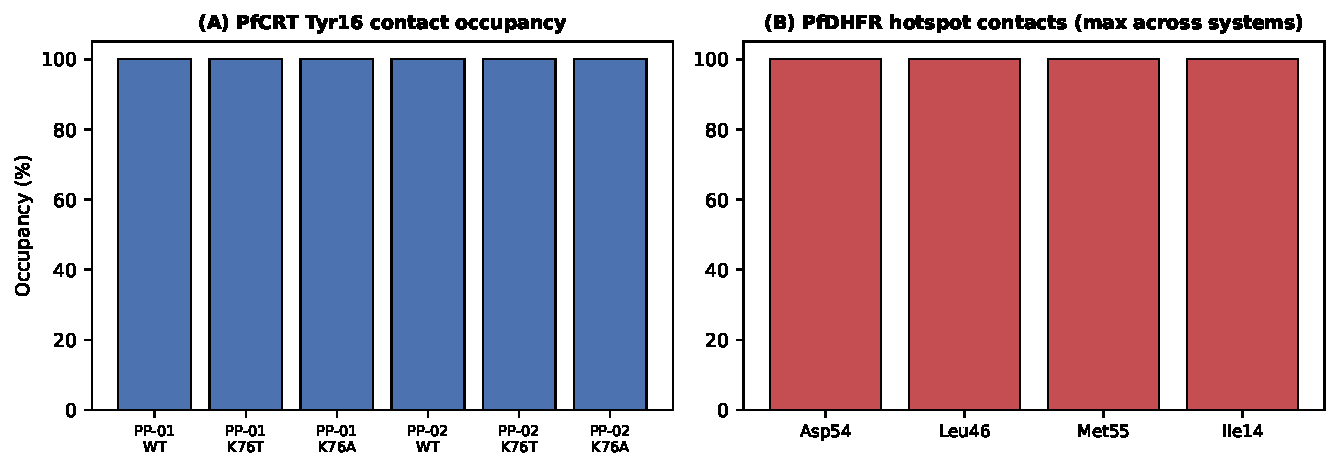
\includegraphics[width=\textwidth]{Graphics/Figure4_ProLIF_Heatmaps.pdf}
\caption{\textbf{Conserved hotspot anchors.} ProLIF interaction-fingerprint occupancy (\num{100} snapshots/system; hydrophobic, van der Waals, and hydrogen-bond contact types). (A) \textit{Pf}CRT Tyr16 contact occupancy per system: \qty{100}{\percent} in five of six PfCRT systems. (B) \textit{Pf}DHFR hotspot contacts (Asp54, Leu46, Met55, Ile14): maximum occupancy across the PP-01/PP-02 states. Source: ProLIF interaction-fingerprint analysis of the QC-PASS trajectories.}
\label{fig:prolif_heatmaps}
\end{figure}

\subsection{Orthogonal Multi-Dimensional Triage}

RRS, ACSI, and PNS show non-significant pairwise associations on the primary cohort ($n=\num{12}$; $\rho \in [-0.41, -0.21], p_{\text{adj}} > 0.50$; \cref{tab:crossmetric}), consistent with distinct ranking dimensions. In an exploratory post hoc check, controlling for molecular weight and scaffold frequency gave a moderate partial PNS--RRS association ($\rho_{\mathrm{partial}} = -0.6154$, descriptive only, no formal test); it does not overturn the pre-declared null result above.

STRING threshold sensitivity (confidence cutoffs 400, 700, 900) showed stable PNS ranks ($\rho$ \numrange{0.9632}{0.9975}; 400-vs-700 \num{0.9975}, 700-vs-900 \num{0.9681}, 400-vs-900 \num{0.9632}). Threshold choice therefore does not alter ranking within this panel. This differs from the PfCRT-centrality imputation sensitivity (\cref{SM-tab:s7_pns_sensitivity}).

Explicit-solvent MD evaluates dynamic stability without reliance on training distributions, providing a complementary check on static scores.

\subsection{Mechanistic Context and Multi-Target Positioning}

The retained PfCRT poses are consistent with microsecond-scale transporter studies \citep{tanner2025pfcrt}: Lys76 anchors the central cavity, and K76T/K76A alter local charge density and hydration, permitting ligand reorientation that preserves hydrophobic contacts despite grid-level penalties.

Within a single-drug--multi-target framing \citep{polypharmacology_malaria_2026}, Class-A* candidate PP-01 is prioritized for assay follow-up: it retained multi-target binding potential across mutant landscapes in these simulations. Whether dual-target engagement raises any evolutionary barrier to resistance cannot be determined computationally. It requires prospective biochemical, structural, and \textit{in vitro} evaluation. We make no resistance, fitness, or evolutionary claim; PP-15, a wild-type probe outside the Set-C estimand, carries no such interpretation.

\subsection{Practical Guidance}

The combined results translate into four operational rules for resistance-aware triage pipelines. (i) Do not rank resistance variants by rigid-receptor $\Delta\Delta G$ alone: it failed both an external enrichment benchmark (DEKOIS 2.0 PfDHFR ROC-AUC \num{0.450}) and a retrospective phenotype comparison ($\rho$ \numrange{-0.13}{0.19}). (ii) Treat disagreement between static docking and short explicit-solvent MD as a flag for experimental follow-up rather than as evidence against either method, consistent with established MD-based pose filtering \citep{liu2017mdfilter}. (iii) Report RRS, PNS, and ACSI as separate descriptive dimensions rather than combining them into a single index, given their non-significant mutual associations at cohort scale. (iv) Enforce the WT-eligibility gate ($|S_{\mathrm{WT}}| \ge \qty{5.0}{\kcalmol}$) before computing any ratio-based score, to prevent inflation on weak wild-type baselines. \Cref{tab:claim_ledger} states, for each central claim of this study, the evidence and its status under the analyses reported here.

\begin{table}[htbp]
\centering
\caption{\textbf{Claim ledger.} Evidential status of the central claims under the analyses reported in this study. Statuses are scope-qualified: ``supported'' means supported within the declared protocol and sampling limits, not validated prediction.}
\label{tab:claim_ledger}
\scriptsize
\begin{tabular}{@{}p{0.32\textwidth} p{0.42\textwidth} p{0.15\textwidth}@{}}
\toprule
Claim & Evidence reported here & Status \\
\midrule
Static docking and short MD estimate the same target quantity & 7/8 matched mutant states diverge; 95\% Wilson CI \qtyrange{52.9}{97.8}{\percent} excludes \qty{50}{\percent} chance ($n=\num{8}$) & Refuted at this scope \\
Vina enriches near-native poses on DEKOIS 2.0 \textit{Pf}DHFR & ROC-AUC \num{0.450}; $\mathrm{EF}_{5\,\%} = \num{0.00}$ (chance level) & Refuted \\
Rigid-receptor $\Delta\Delta G$ tracks resistance fold-shifts & ChEMBL: $\rho$ \numrange{-0.13}{0.19}; direction agreement \qtyrange{28.6}{41.7}{\percent} & Refuted \\
RRS, PNS, and ACSI are mutually independent discriminant dimensions & $\rho \in [-0.41, -0.21]$, $p_{\mathrm{adj}} > 0.50$ ($n=\num{12}$) & Not supported \\
Class assignments survive independent rescoring & GNINA \qty{100}{\percent} agreement but Class-A fraction \num{0.974} & Supported, near-degenerate \\
\textbf{PP-01} retains poses across matched mutant states & 8/8 QC-PASS (6 matched mutant states); bound fraction \num{1.000} in \qty{10}{\ns} trajectories & Supported (protocol-local) \\
MM-GBSA endpoint resilience (K76T, C59R) & Within the \qty{2.01}{\kcalmol} WT noise floor; K76A sensitivity \qty{7.75}{\kcalmol} & Supported at pilot scope; no claim for K76A \\
Multi-target engagement raises an evolutionary barrier to resistance & Not determinable computationally & Open (prospective) \\
\bottomrule
\end{tabular}
\end{table}

\subsection{Limitations}

\begin{enumerate}
    \item \textbf{Receptor models:} mutant structures are homology models (quality criteria in Methods), not experimental structures.
    \item \textbf{Timescale and replication:} per JCIM guidelines \citep{soares2023mdreport}, the \qty{10}{\ns} single-replicate pilot is a structural stress test, not a converged free energy or residence-time measurement. The PP-01 PfCRT K76A endpoint (\qty{-35.29}{\kcalmol}) differs by \qty{7.75}{\kcalmol} from a second trajectory (\qty{-27.54}{\kcalmol}; \cref{SM-tab:s19_k76a_replicate}), which exceeds the \qty{2.01}{\kcalmol} WT noise floor. We therefore make no endpoint resilience claim for K76A.
    \item \textbf{Sample size:} primary two-target cohort $n=\num{12}$, plus 5 single-target candidates and a 39-ligand external panel.
    \item \textbf{Protonation:} preparations at physiological pH; PfCRT dynamics in the acidic digestive vacuole (pH~\num{5.2}) may differ.
    \item \textbf{Retrospective experimental reference:} the ChEMBL comparison (\cref{SM-tab:s20_chembl_foldshift}) rests on whole-parasite IC$_{50}$ values from non-isogenic DHFR-genotyped strains; it is a descriptive phenotype-level reference, not enzyme-level or cohort-specific validation. No experimental measurement was performed on the Set-C candidates, which therefore remain without their own experimental anchor. ChEMBL docking used a single seed (\num{42}).
\end{enumerate}

% ============================================================================
% 5. CONCLUSION
% ============================================================================

\section{Conclusion}

This study reports a resistance-aware computational triage workflow for African antimalarial natural products. Static grid docking ($\Delta G_{\mathrm{grid}}$) and short explicit-solvent MD pose retention ($\mathrm{MD\text{-}RRS}_{\mathrm{distance}}$) capture distinct, non-equivalent signals: dynamic pocket accommodation retained poses where static docking predicted penalties in 7/8 matched mutant states (95\% Wilson CI \qtyrange{52.9}{97.8}{\percent}, $n=\num{8}$). The multi-metric descriptors stayed mutually non-associated at cohort scale ($\rho \in [-0.41, -0.21]$, adjusted $p > 0.50$), so we report them as distinct descriptive dimensions rather than a combined index. \textbf{PP-01} (Class A*) showed multi-target engagement across PfDHFR and PfCRT mutant panels and passes the two-target pilot gate (Class-A* retention plus pose retention in matched mutant trajectories). Whether this implies any elevated evolutionary barrier requires prospective biochemical, structural, and \textit{in vitro} evaluation; these findings prioritize specific natural product scaffolds for that testing. External checks bounded the docking estimand at chance level (DEKOIS 2.0 PfDHFR ROC-AUC \num{0.450}; ChEMBL direction agreement \qtyrange{28.6}{41.7}{\percent}), and no experimental measurement was performed on the Set-C candidates themselves.

% ============================================================================
% BACK MATTER
% ============================================================================

\section*{Authors' Contributions}

Myke Vital Sao Temgoua: Methodology, software, formal analysis, investigation, data curation, writing -- original draft. Jean-Pierre Tchapet Njafa: Methodology, software, supervision, writing -- review \& editing. Penabei Samafou: data curation, writing -- review \& editing. Wilfred Fon Mbacham: conceptualization, validation, writing -- review \& editing. Serge Guy Nana Engo: conceptualization, methodology, supervision, writing -- review \& editing. All authors read and approved the final manuscript.

\section*{Data Availability}

Docking results, metric outputs, analysis scripts, and source-data records are publicly archived on Zenodo (dataset CC-BY-4.0; analysis code MIT) at \href{https://doi.org/10.5281/zenodo.22829031}{DOI: 10.5281/zenodo.22829031}. Large parent-study trajectories are excluded; conclusions are restricted to the trajectory-derived summaries reported above. The retrospective ChEMBL comparison (curated paired IC$_{50}$ inputs with assay provenance, \num{112} docking scores, analysis outputs, and a script and parameter hash manifest) is archived with the source-data records. The parent-study ligand identity review (production-ligand composition, numbering provenance, and receptor-correspondence checks) is archived with the same records.


\section*{Competing Interests}

The authors declare no competing interests.

\section*{Acknowledgements}
Computational resources were provided by the penavoraserver cluster (ThinkStation P720, \qty{128}{\giga\byte} RAM, \num{48} cores). We acknowledge the SWISS-MODEL server and the GROMACS development team. This research received no specific grant from any funding agency.

During the preparation of this manuscript in September 2026, the authors utilized AI tools to support code review, provide structured text suggestions, and perform consistency checks. The authors designed all analyses, maintained full control over the scientific interpretation, and rigorously verified all computational results and quantitative claims against the original source records.



\section*{Supporting Information}
Docking enrichment and homology-model quality tables; P2Rank box audit; MPO, ADMET, and ACSI sensitivity; RRS radar profiles and threshold sensitivity; PNS imputation and Tartarus calibration; cohort and evidence-scope tables; PlasmoDB identifiers; parent-study and Set-C pilot MD/MM-GBSA summaries; robustness and upstream-workflow-context tables; retrospective ChEMBL genotype--phenotype fold-shift table (PDF).


% ============================================================================
% BIBLIOGRAPHY
% ============================================================================


\bibliographystyle{unsrtnat}
\bibliography{P2_V2609C_bibliography}

\end{document}
